\chapter{Python}
\thispagestyle{fancy}
\lstset{language=Python}

The official python documentation can be found at the following links
\begin{lstlisting}
# Documentation for version 3+
https://docs.python.org/3/
# Documentation for version 2+
https://docs.python.org/2/
\end{lstlisting}


\section{Imports and libraries}

On Linux, there's a site-packages folder that imported libraries are all in. These are located in the following directories for python versions 2.7 and 3.6 respectively.

\begin{itemize}
	\item /usr/lib/python2.7/site-packages
	\item /usr/lib/python3.6/site-packages
\end{itemize}

I believe you only have specify the path from that folder on. For example, an app that uses the import program.script.interface as interface will have the interface.py file installed to usr/lib/python3.6/site-packages/program/scripts.

\section{Basics of Python}

Import floating point division which allows python 2 compatibility when using division with doubles. Include this at the beginning of the script.
\begin{lstlisting}
from __future__ import division
\end{lstlisting}



\section{Program parameters}

You can add input parameters for a python script/program using the argparse package.
\begin{lstlisting}
import argparse

parser.add_argument(
		'-v',							# Creats a parameter with -v
		'--verbose',					# Creates args.verbose parameter
		required=False,					# Sets the parameter to not required.
		default=False,					# Sets default value
		action='store_true',			# Sets value to true if supplied
		help="Enables verbose mode.")	# Sets help message
					
parser.add_argument(
		'-i',							# Creates a parameter with -i
		'--input',						# Creates args.input parameter
		required=True,					# Sets the parameter to be required
		default="potato",				# Sets default value to "potato"
		help="An input string ot use")	# Sets a help message
		
if args.input is not none:
	print("Input value is {0}".format(args.input)) # prints the input value.
	
if args.verbose:
	print("Verbose is on!")
\end{lstlisting}





\section{Methods and Functions}

To create a method with some parameters you can do the following
\begin{lstlisting}
def methodName(parameter1, parameter2):
	"""
	This is a description of the method
	:param parameter1: some value
	:param parameter2: some other value
	:return a, b - description of what is returned.
	"""
	
	# You can return multiple values
	return parameter1, parameter2	
\end{lstlisting}



\section{String manipulation}

To split a string by a \textbf{delimiter}\index{delimiter} you can use the following
\begin{lstlisting}
stringValue = "Test;string"

firstPart = stringValue.split(';')[0] 	# Stores "Test"
secondPart = stringValue.split(';')[1]	# stores "string"
\end{lstlisting}



\section{Arrays and lists}

To check if any value in one array/list is in another array/list, you can use any().
\begin{lstlisting}
list = ["list", "of", "strings"]
items = ["second", "list", "of", "things"]

if any(thing in list for thing in things):
	print("There is an item in items also in list")
else:
	print("Something is broken")
\end{lstlisting}



\section{Plotting and Graphs\index{Plotting and Graphs}}

A nicely formatted plot with a legend using the pylab package.
\begin{lstlisting}
import pylab as plt #Imports the correct packages for plotting.

plt.title('Contamination & Beam Health % vs Time') # Creates a title.

plt.plot(t, Contamination, '-b', label='Contamination') #Plots Contamination in blue.
plt.plot(t, Beam_loss, '-r', label='Beam Loss') #Plots Beam_loss in red.
plt.plot(t, Beam_health, '-g', label='Beam Health') #Plots Beam_health in green.
#plt.plot(x,y,'-color', label='Legend Label') #Template

plt.xlabel("time (seconds)") #Creates a x-axis label
plt.ylabel("Contamination %") #Creates a y-axis label

plt.legend(loc='center right') #Creates a legend with the labels set above.
#Other locations include upper/lower/center left/right

plt.show() #Displays plot.
\end{lstlisting}
This code would display a graph such as the one below such that the proper values are input.

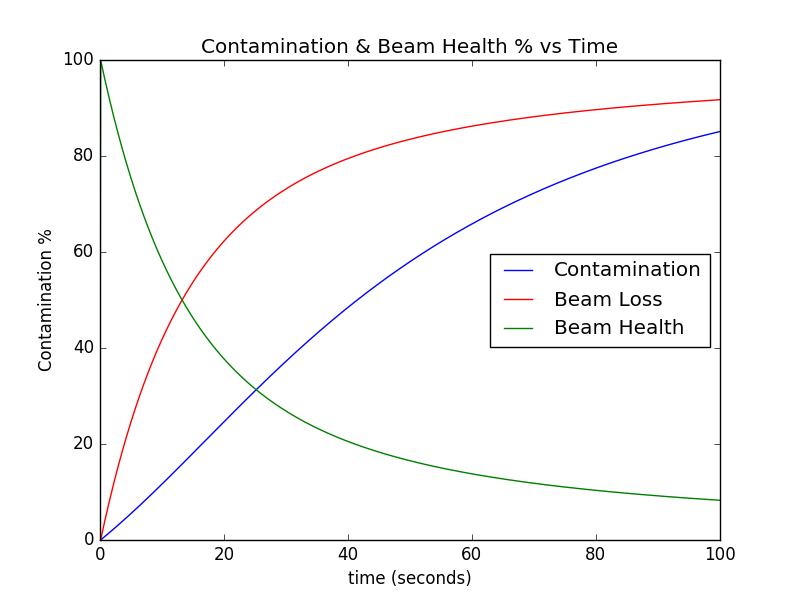
\includegraphics[width=0.5\linewidth]{./Images/Figures/figure_1-4}


A nicely formatted plot with a legend using the matplotlib package.
\begin{lstlisting}
import matplotlib as plt #Imports the correct packages for plotting.

fig = plt.figure(dpi=1200) # increase resolution of the plot.
plt.scatter(x, y, s=0.1) # +Plot x data vs y data with a dot size of 0.1
fig.suptitle(title, fontsize=12) # adds a title to the figure

plt.xlabel("x axis label") # Creates a x-axis label
plt.ylabel("y axis label") # Creates a y-axis label

manage = plt.get_current_fig_manager()
manage.full_screen_toggle() # makes the plt full screen.

plt.show() # Displays plot.
plt.savefig("fileName.png") # Saves the figure as an image
\end{lstlisting}

